\chapter{IoT Malware Laboratory}
In order to successfully complete the laboratory activity, it is strongly advised to use the provided virtual machine. The credentials of the root user are \texttt{mirai:mirai}, this user contains all the necessary information to complete the laboratory. The virtual machine is based on Lubuntu 20.04 LTS, from which unnecessary software has been removed, to make the system lighter and Wireshark was installed. The whole lab experience can be performed without giving the machine internet access. \\
The first four exercises have the objective of providing a hands-on experience with the Mirai botnet from the point of view of an attacker who decides to download the source-code and create his own instance.

\section{Mirai botnet initialization}
We decided to use Docker since it provides a lightweight way to create machines that can act both as servers and clients. We also decided to use \texttt{docker compose} since it allows us to define and run multi-container Docker applications. To ensure interaction between the containers, we decided to use a custom network to which all the containers are attached. The network is set as \texttt{internal} meaning that the containers do not have access to the internet, we used this approach to ensure that the botnet could not attack any real systems. \\
The first step to start the botnet is to start a terminal and run the following commands:
\begin{enumerate}
    \item \texttt{cd mirai}
    \item \texttt{docker compose up -d}
\end{enumerate}
Since the virtual machine comes with all the Docker images pre-built, the services will start almost instantly. The Mirai botnet can be built to work both with telnet and ssh and both in debug and release mode. We opted on using the telnet version, built in debug mode to have unencrypted traffic and to have a better understanding of the botnet's behavior.
This commands will start some docker containers with the following services:
\begin{itemize}
    \item The CNC server (Ubuntu) with the database (MySQL)
    \item 4 containers (Alpine) simulating IoT devices. These four devices are running a telnet server.
    \item A Nginx container to simulate a website (victim)
\end{itemize}
To actually start the botnet, the following command must be executed:
\begin{itemize}
    \item \texttt{docker exec -it mirai-cnc bash /home/cnc/starter.sh}
\end{itemize}
This command will start the CNC server allowing connections from both the bots and the attacker. It is important to notice that the CNC server is running on a fixed IP address which is \texttt{192.168.10.10} and that it is possible to access the CNC server from the host machine by using telnet. The CNC server implements a telnet server in GO from which it is possible to interact with the botnet.

\begin{figure}
    \centering
    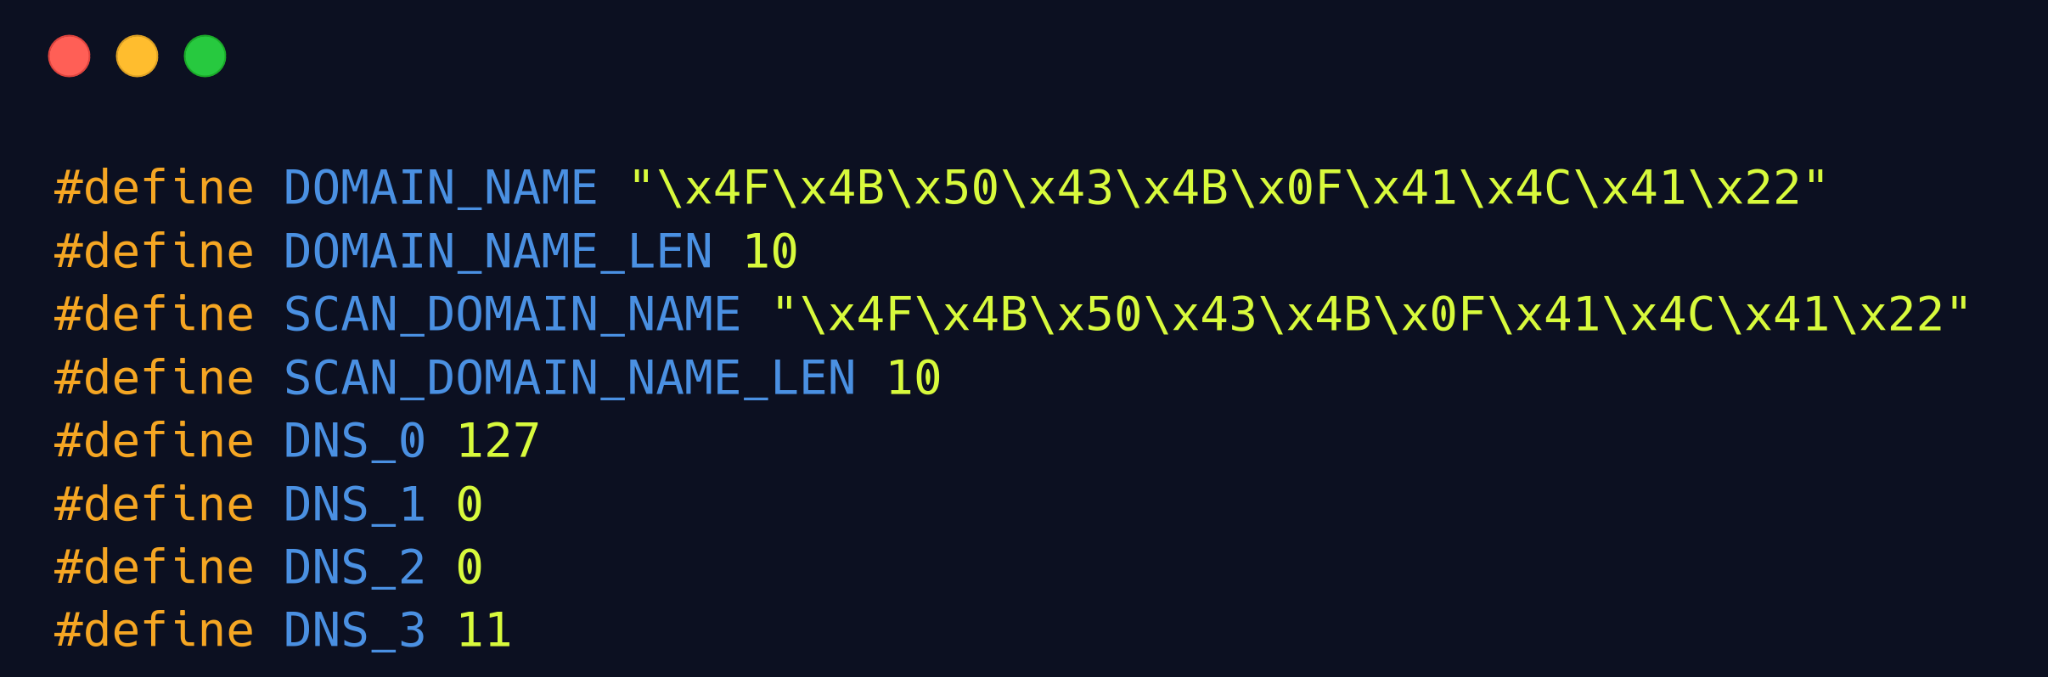
\includegraphics[width=0.8\textwidth]{resources/images/config.png}
    \caption{config.h file}
    \label{fig:config_h}
\end{figure}
\section{Exercise 1: Find the CNC}
\label{section:ex1}
Each bot that is part of the Mirai botnet reports to the CNC its status and waits for commands from it, this means that the bot has to know at any time which how to contact the CNC (IP address and port). To achieve this the bot has the value of a DNS entry which resolves to the CNC IP address hard coded in the binary. The actual entry can be found in the file \texttt{bot/config.h} (figure \ref{fig:config_h}) with name \texttt{DOMAIN\_NAME}. In the same config file it is possible to find also the \texttt{SCAN\_DOMAIN\_NAME} entry which refers to the reporting server to which the bot sends information about the newfound victims, in this case it is the same as the CNC. Together with these entries the bot is also provided with four entries whose name starts with \texttt{DNS\_} that are used to indicate the DNS server's address\footnote{In our case the IP is set to 127.0.0.11 which is the address of the Docker internal DNS}. The actual algorithm to encrypt these entries can be found in the file \texttt{tools/enc.c}, it basically reduces to splitting the key in four parts and using them to XOR each character of the entry. This is probably done to protect the CNC since it would be easy for someone to get the IP address of the CNC by just intercepting the traffic or reversing the binary, and while it is really easy to change an IP address it would be way harder to change the DNS server's address since it is hard coded in the binary.

\section{Exercise 2: Connect to the CNC}
Since the entire infrastructure is run in some containers on the host machine there are two possible ways to connect to the CNC server. The first one employs the usage of the telnet command run from the host machine, \texttt{telnet 192.168.10.10} will connect to the CNC server. To check that the CNC IP is actually \texttt{192.168.10.10}, the command \texttt{docker ps} can be run to see the list of running containers and the command \texttt{docker container inspect mirai-cnc} can be used to see the container's IP address. The second way to connect to the CNC server is to run the telnet command from the CNC server itself, this can be done by running the command \texttt{docker exec -it mirai-cnc telnet localhost}. The credentials of the only existing account are \texttt{root:root}. Once inside the CNC server it is possible to use the `?' command to list the possible attacks, and since we are logged in as a privileged user it is possible to use two additional commands \texttt{adduser} which adds a user to the CNC server and \texttt{botcount} which returns the number of bots connected to the CNC server. The \texttt{botcount} command was slightly modified to return the IP addresses of the bots connected to the CNC server together with their number.

\section{Exercise 3: Spread Mirai}
This exercise has the objective of infecting some containers with the Mirai malware, to achieve this the idea is to get access to one of the IoT devices and then use it to infect the other devices. The target device has IP \texttt{192.168.10.5}. All the IoT devices have the same credentials which are \texttt{admin:admin1234}, they were originally found in a made up manual page which can be found in our repository at \texttt{/report/resources/pdf}\footnote{\url{https://github.com/luiss07/mirai/tree/main/report/resources/pdf}}. Since the CNC together with the telnet interface provides an endpoint to download files it can be used as the loader server. The first step is to connect to the target machine using the command \texttt{telnet 192.168.10.5}, after logging in it is possible to get the actual scanner script from the CNC by using the command \texttt{wget mirai-cnc/bins/scanner.py}. There are a few things to consider here, the first one is that instead of the IP it is possible to use the container name \texttt{mirai-cnc} since we are inside a docker container in the same network. The other important thing to notice is that we decided to reimplement the scanner because the original scanner targets random machines over the internet. The scanner script is written in python and tests a set of credentials against some known IPs. If the scanner is run as-is it would not connect to any device since it is missing the credentials used by the devices. To solve this issue the script must be updated either from the CNC server or from the host machine. If the CNC route is chosen the file can be found in the folder \texttt{/var/www/html/bins/}, after editing it, downloading it again on the target machine and running it three machines will be infected. It is possible to verify the infected machines from the CNC Telnet interface, by using the \texttt{botcount} command. Even though there are four potential victims only three of them will be infected, this is due to a programming error on our side which led to the scanner not targeting the machine with IP \texttt{192.168.10.5}.

\begin{figure}
    \centering
    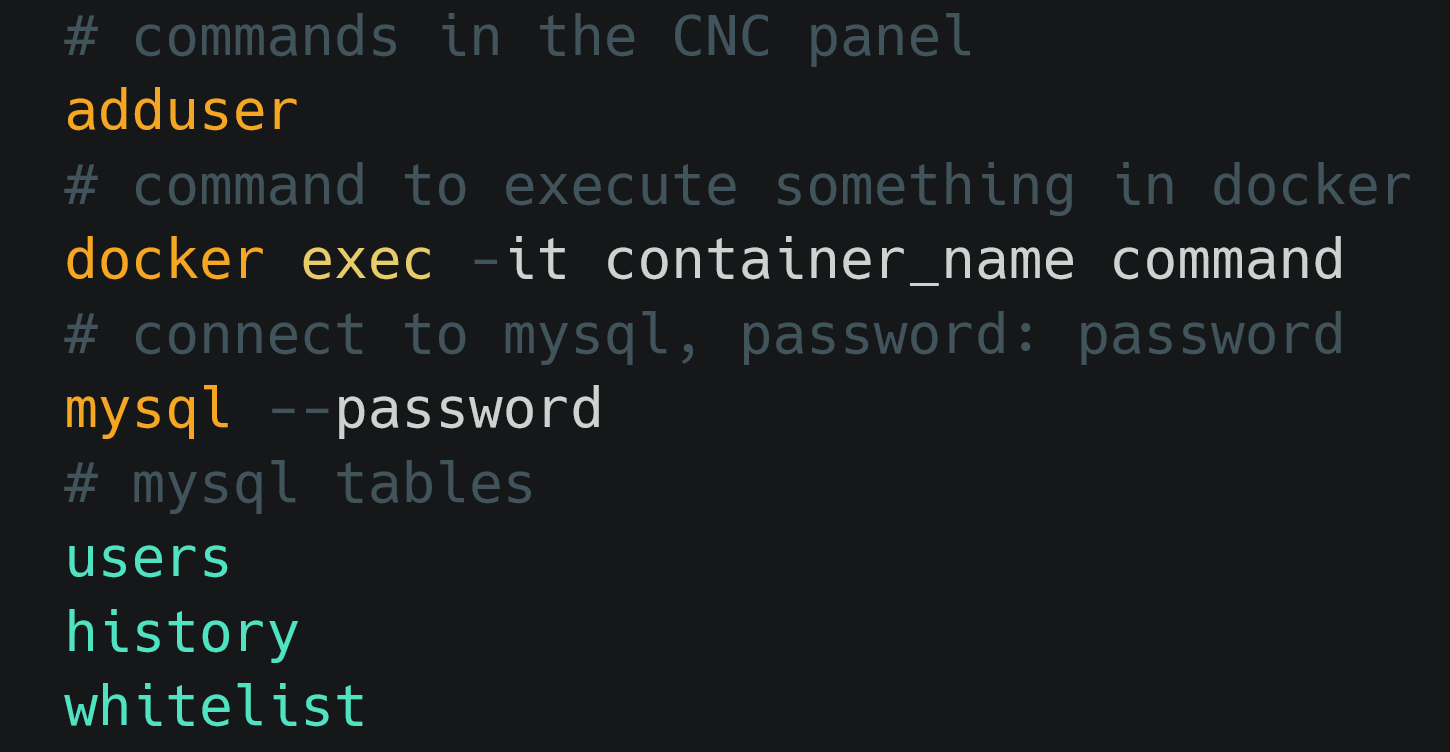
\includegraphics[width=0.8\textwidth]{resources/images/create_user.png}
    \caption{Commands needed for the fourth exercise}
    \label{fig:database}
\end{figure}

\section{Exercise 4: Sell the service}
This optional exercise was created to show how it is possible to create a new user account inside the CNC. All the necessary information to perform this exercise can be found in figure \ref{fig:database}. The first step is to connect to the CNC server using telnet and logging in as the \texttt{root} user. By using the \texttt{adduser} command the credentials and constraints for the new user can be inserted, an example of this can be found in figure \ref{fig:add_user}. It is important to notice that if no constraint is provided the CNC will not give any error, but the user will not be created. After creating the user it is possible to check the database to check how the user information are stored. The first step to achieve this is to connect to the MySQL database found in the CNC server, this can be done by running the command \texttt{docker exec -it mirai-cnc mysql -password}, the password is \texttt{password}. Once inside the MySQL shell it is possible to run the command \texttt{use mirai} to select the database and then \texttt{select * from users} to see the table containing the users. The result of this command can be found in figure \ref{fig:table_users}. One interesting thing to notice is that the password is stored in plain text by the original implementation. This is a bad practice and should never be done in a real-world scenario since an attacker compromising the database would have access to the all the accounts. To avoid this issue hashing is used in real-world applications, this way even if the attacker gets access to the database he would not be able to get the actual password. \\
Together with the user accounts the database also stores a list of \texttt{whitelisted} IPs which the bots will not attack and a table which contains the log of all the attacks launched by the botnet.

\begin{figure}
    \centering
    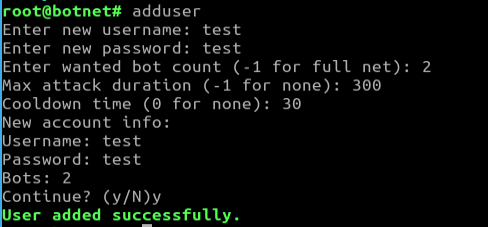
\includegraphics[width=0.8\textwidth]{resources/images/add_user.png}
    \caption{Result of the adduser command}
    \label{fig:add_user}
\end{figure}

\begin{figure}
    \centering
    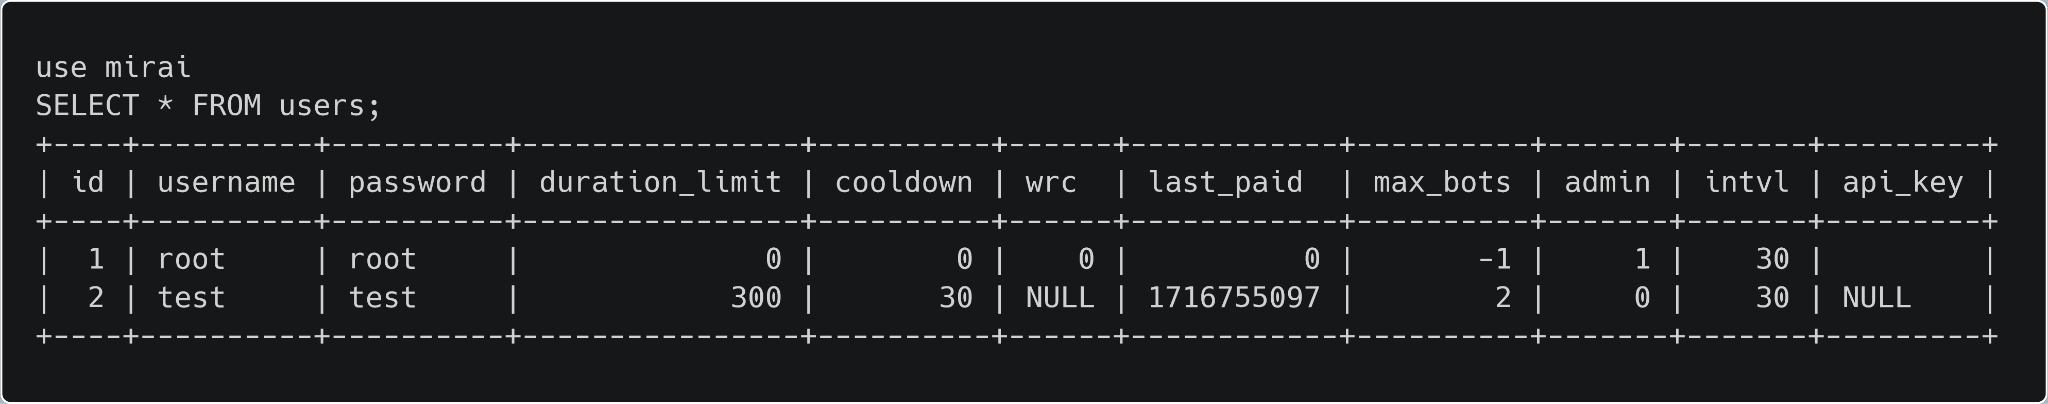
\includegraphics[width=1.0\textwidth]{resources/images/table_users.png}
    \caption{Database content after adding the new user}
    \label{fig:table_users}
\end{figure}

\newpage
\section{Launch an attack}

From the CNC panel, a specific attack is launched and the network traffic is captured using Wireshark. To initiate an attack, one of the available attack commands listed by the `?' command can be used. The syntax of the command is [attack\textunderscore type] [target\textunderscore ip] [duration], specifying the needed information for the attack.
 
After launching the attack, Wireshark is used to monitor the network traffic. In Wireshark, a message sent from the CNC server to the bots should be observable, found in Figure \ref{fig:wireshark_attack}. This message contains all the necessary information for the bots to execute the attack, including the type of attack, the target IP address, the duration of the attack, and the number of bots involved.

\begin{figure}
	\centering
	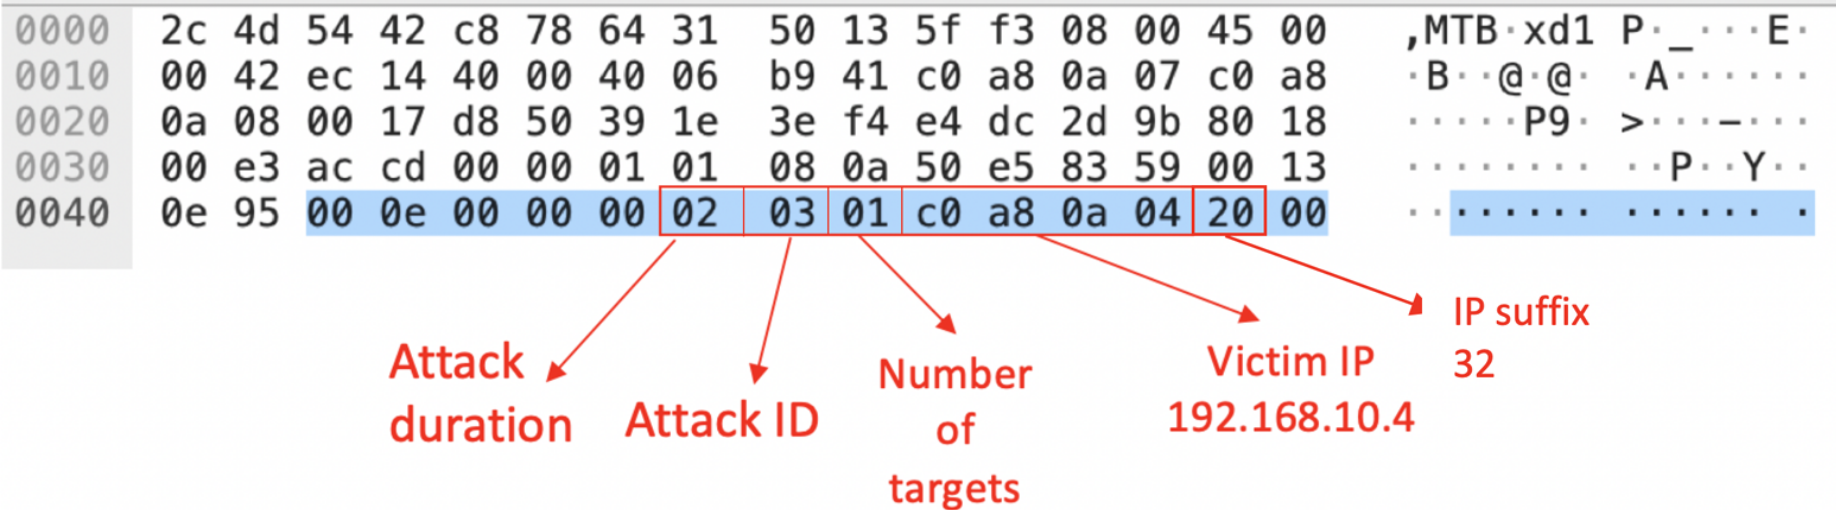
\includegraphics[width=1.0\textwidth]{resources/images/wireshark_attack.png}
	\caption{Packet containing attack information}
	\label{fig:wireshark_attack}
\end{figure}

\section{Exercise 5: Traffic analysis}

In this exercise, different .pcap files containing realistic analyses of Mirai attacks are provided. The scope of the exercise is to examine the packets within each .pcap file and determine which type of attack is represented.
Additionally, there are other .pcap files that, instead of being attacks, represent host and port discovery and brute force of the credentials.

By examining the packets in each .pcap file, key characteristics of different attack types are identified:
\begin{itemize}
	\item \textbf{SYN Flood}: a large number of SYN packets without corresponding ACK responses from the target (Figure \ref{fig:pcap1})
	\item \textbf{HTTP Flood}: a high number of HTTP request packets, sent at a high frequency and with bare minimum content (Figure \ref{fig:pcap5})
	\item \textbf{ACK Flood}: a significant number of ACK packets, typically without corresponding SYN or data packets (Figure \ref{fig:pcap4})
	\item \textbf{UDP Flood}: a high frequency of UDP packets with various source and destination ports (Figure \ref{fig:pcap3})
\end{itemize}

As for the other .pcap files:
\begin{itemize}
    \item \textbf{Host discovery}: multiple ARP packets are sent to discover and map out all possible hosts on a network to identify potential targets for infection and expansion of the botnet (Figure \ref{fig:pcap21})
    \item \textbf{Port discovery}: many SYN packets on different ports of a device to identify open ones, indicating potential vulnerabilities, and potentially locating accessible entry points (Figure \ref{fig:pcap22})
    \item \textbf{Brute force}: within the payload of Telnet packets, Mirai tries different username and password combinations (Figure \ref{fig:pcap6})

\begin{figure}
	\centering
	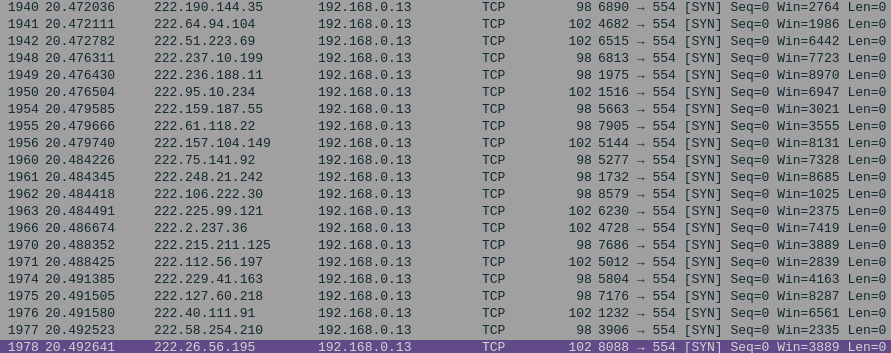
\includegraphics[width=1.0\textwidth]{resources/images/pcap1.png}
	\caption{SYN Flood}
	\label{fig:pcap1}
\end{figure}

\begin{figure}
	\centering
	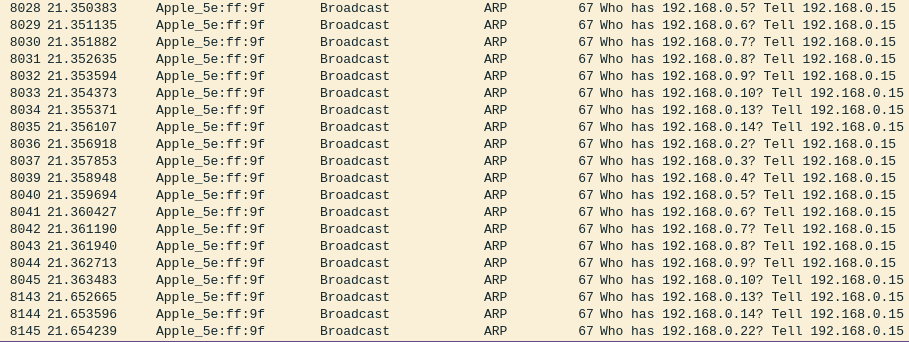
\includegraphics[width=1.0\textwidth]{resources/images/pcap21.png}
	\caption{Host discovery}
	\label{fig:pcap21}
\end{figure}

\begin{figure}
	\centering
	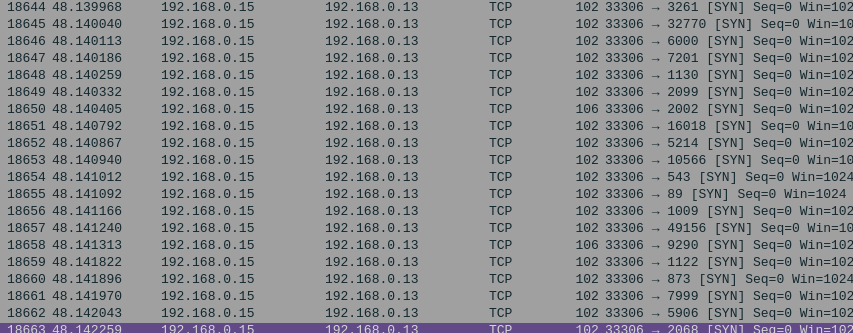
\includegraphics[width=1.0\textwidth]{resources/images/pcap22.png}
	\caption{Port discovery}
	\label{fig:pcap22}
\end{figure}

\begin{figure}
	\centering
	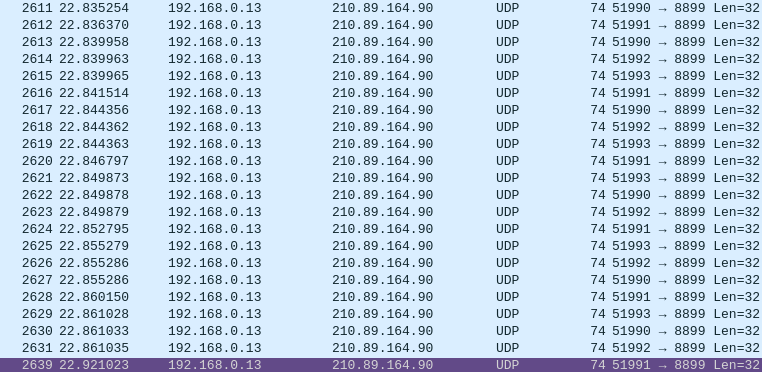
\includegraphics[width=1.0\textwidth]{resources/images/pcap3.png}
	\caption{UDP Flood}
	\label{fig:pcap3}
\end{figure}

\begin{figure}
	\centering
	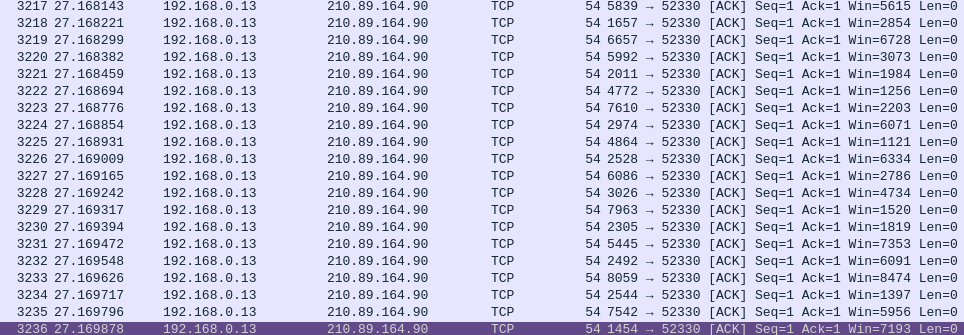
\includegraphics[width=1.0\textwidth]{resources/images/pcap4.png}
	\caption{ACK Flood}
	\label{fig:pcap4}
\end{figure}

\begin{figure}
	\centering
	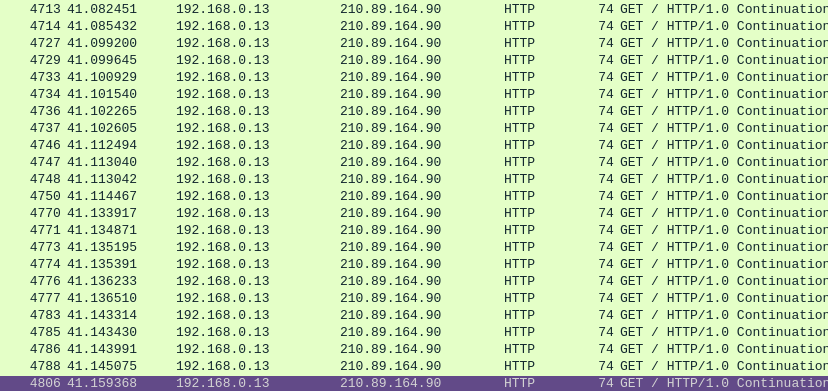
\includegraphics[width=1.0\textwidth]{resources/images/pcap5.png}
	\caption{HTTP Flood}
	\label{fig:pcap5}
\end{figure}

\begin{figure}
	\centering
	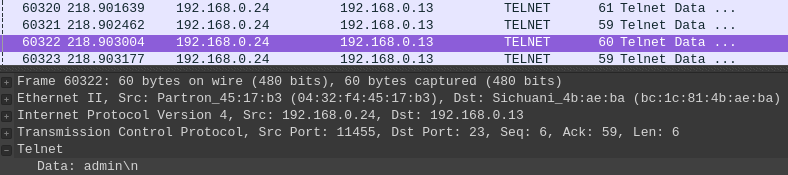
\includegraphics[width=1.0\textwidth]{resources/images/pcap6.png}
	\caption{Brute force}
	\label{fig:pcap6}
\end{figure}
